\documentclass[11pt]{beamer}
\usetheme{Copenhagen}
\usepackage[utf8]{inputenc}
\usepackage[french]{babel}
\usepackage[T1]{fontenc}
\usepackage{amsmath}
\usepackage{amsfonts}
\usepackage{amssymb}
\usepackage[font=small,labelfont=bf]{caption}
\usepackage{tcolorbox}
\usepackage{graphicx}
\newtcolorbox{mybox}[1]{colback=blue!5!white,colframe=blue!60!black,fonttitle=\bfseries,title=#1}
\author{ADOLPHE Benjamin - BERJOLA Matthias}
\setbeamercovered{transparent} 
\setbeamertemplate{navigation symbols}{} 
\setbeamertemplate{headline}{}
%\logo{} 
\institute{Université de la Réunion} 
%\date{} 
%\subject{} 
\begin{document}

\begin{frame}
\title{Planee application de gestion d'évènements}
\titlepage
\end{frame}



\begin{frame}{Introduction}
\section{Introduction}

\begin{itemize}
\onslide<1-3>{\item[•] Le contexte}
\onslide<2-3>{\item[•] L'idée}
\onslide<3>{\item[•] le plan d'action}


\end{itemize}

\end{frame}






\begin{frame}{Plan}
\begin{itemize}
\item[•] Description de l'application  \pause
\item[•] Architecture de l'application \pause
\item[•] Problèmes rencontrés  

\end{itemize}
\end{frame}



\begin{frame}{Description de l'application}
\section{Description de l'application}
\begin{itemize}
\item[•] Planee c'est quoi ? \pause
\end{itemize}
\begin{mybox}{Une application de gestion d'évènement complet}
une application de gestion d'évènements de A à Z, allant de la commande des fleurs à la réservation de salles.
	
\end{mybox}
\pause
\begin{itemize}
\item[•] Un projet innovant \pause
\end{itemize}
\begin{mybox}{Du jamais vu}
Contrairement aux applications de gestions habituel on peut tout programmer depuis son téléphone 
	
\end{mybox}



\end{frame}


\begin{frame}{Architecture de l'application}
\section{Architecture de l'application}
4 activités: 
\begin{itemize}
\onslide<1,5>{\item[•] MainActivity}
\onslide<2,5>{\item[•] AddActivity}
\onslide<3>{\item[•] DetailActivity}
\onslide<4>{\item[•] UpdateActivity}
\end{itemize}
\end{frame}

\begin{frame}{MainActivity}
\begin{columns}
\column{0.35\textwidth}
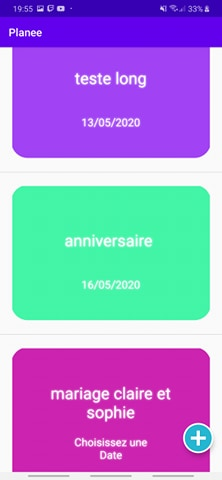
\includegraphics[scale=0.4]{HomeWEvents1}

\column{0.35\textwidth}
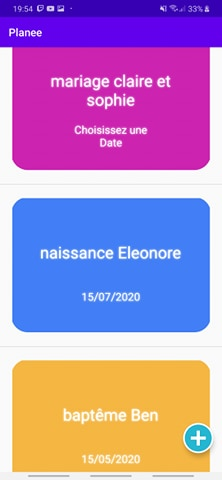
\includegraphics[scale=0.4]{HomeWEvents2}

\column{0.35\textwidth}
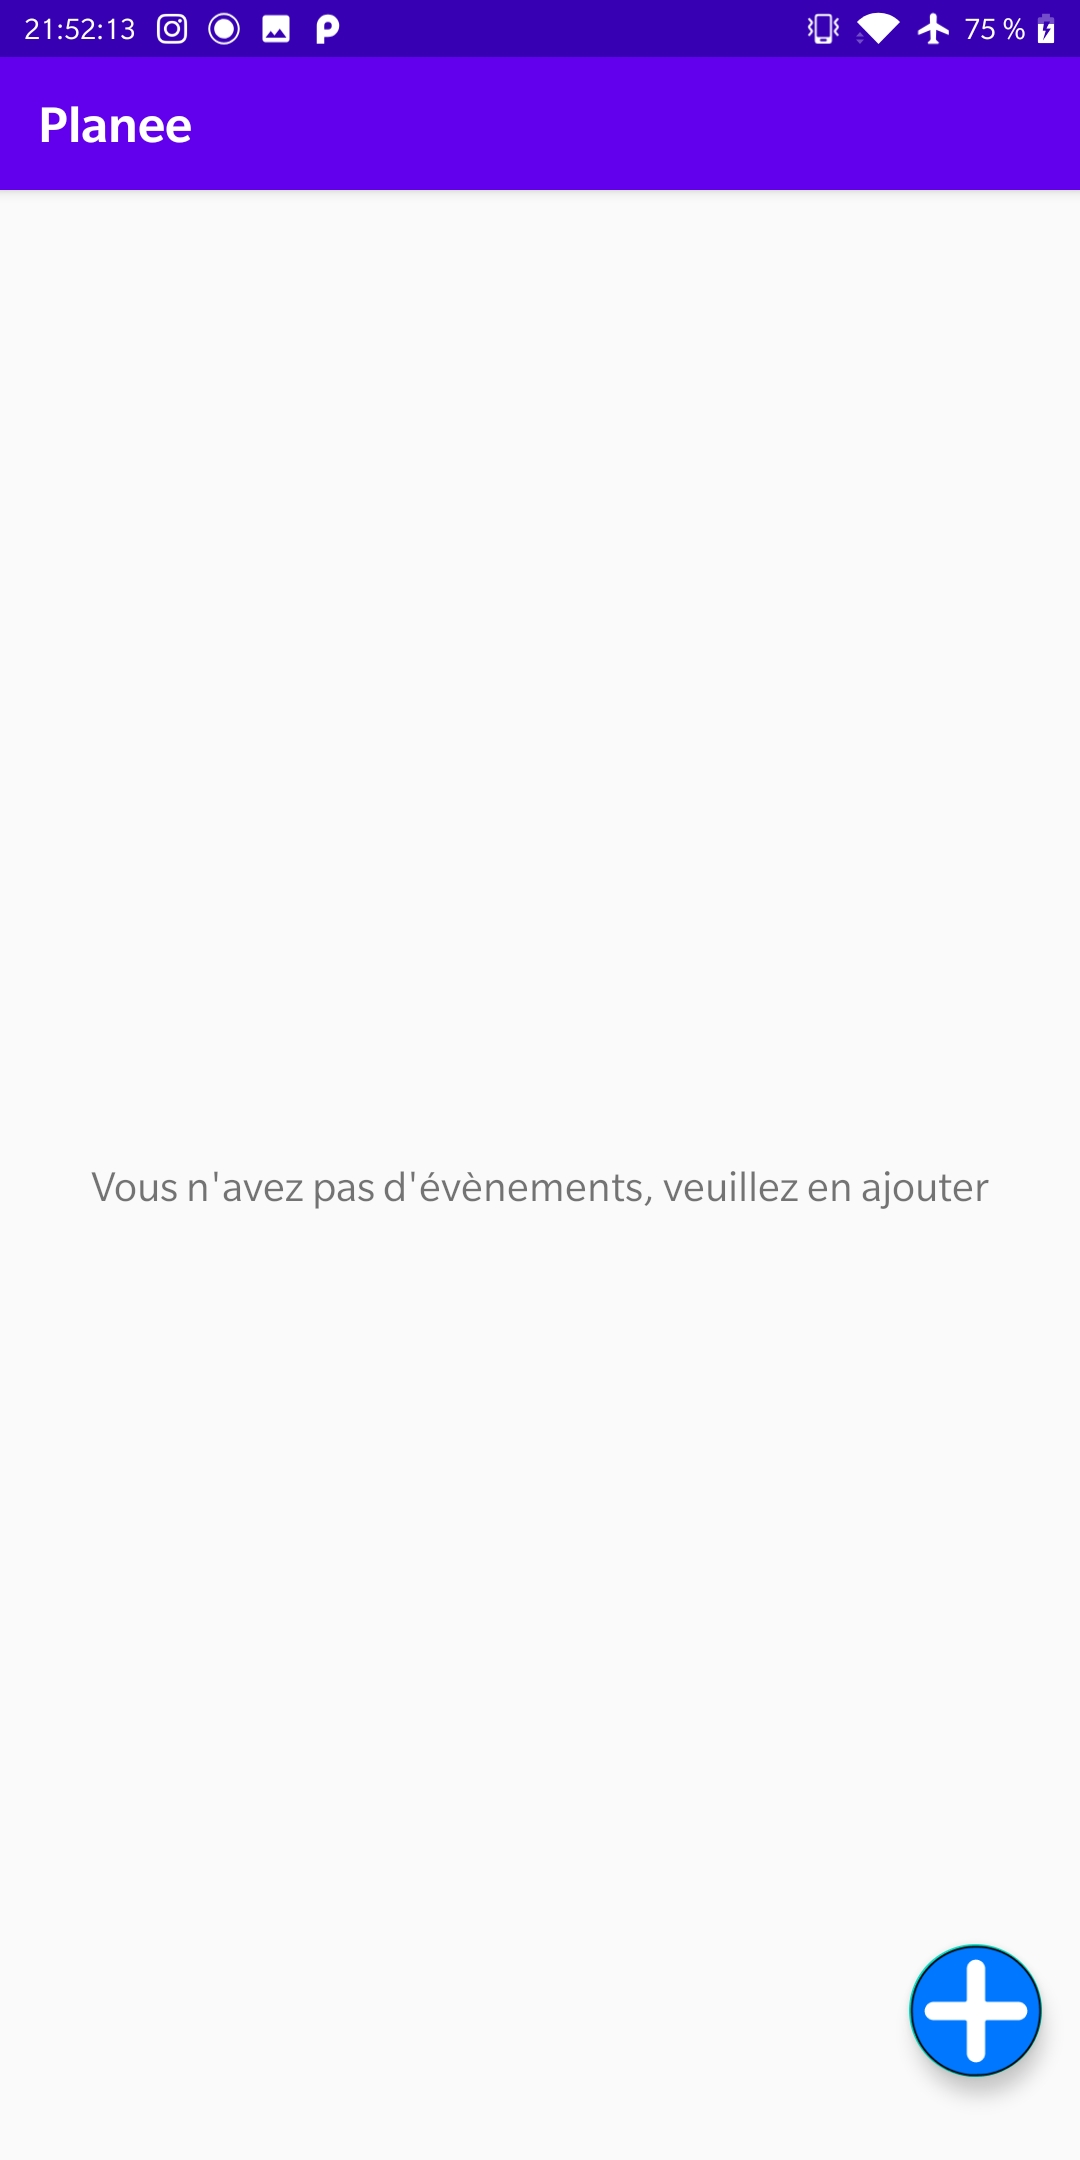
\includegraphics[scale=0.1]{ListViewNoEvent}
\end{columns}

\end{frame}

\begin{frame}{AddActivity}
\begin{columns}
\column{0.5\textwidth}
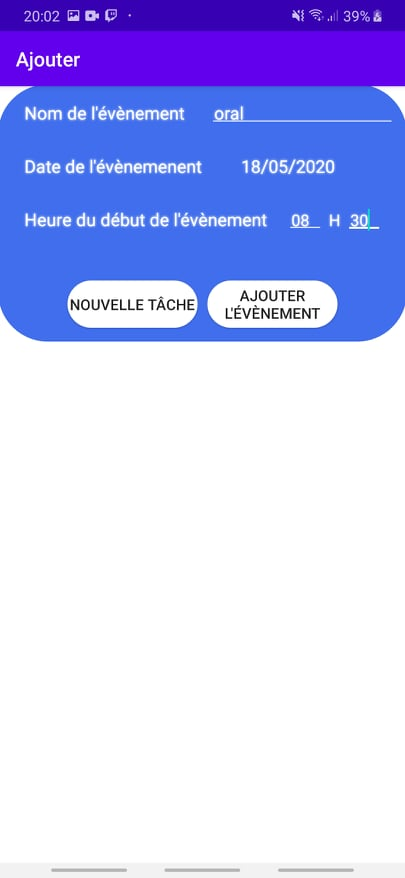
\includegraphics[scale=0.4]{FormNoTask}

\column{0.5\textwidth}
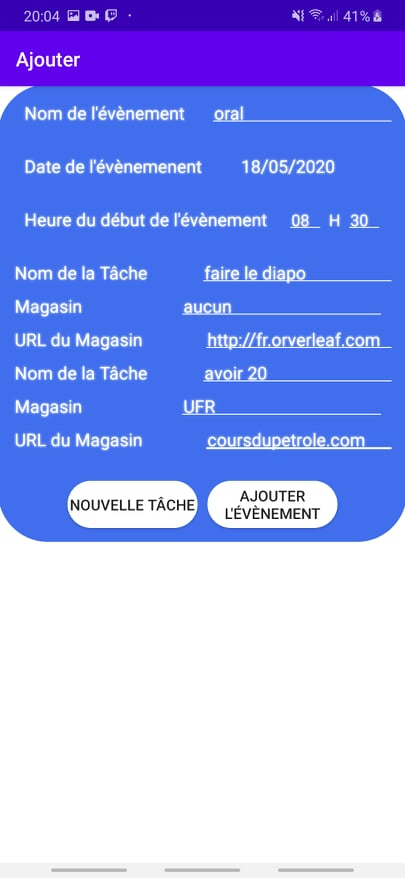
\includegraphics[scale=0.4]{FormWTask}

\end{columns}

\end{frame}


\begin{frame}{Problèmes rencontrés}

\section{Problèmes rencontrés}
\begin{itemize}
\item[•] Problèmes liés aux fragments\pause
\item[•] Problèmes liés aux Layouts\pause
\item[•] Problèmes liés aux Notifications
\end{itemize}

\end{frame}



\begin{frame}{Problème Rencontrés}

\begin{mybox}{Problèmes liés aux fragments}
\onslide<1-3>{2 problèmes majeurs: }
\begin{itemize}
\onslide<2,3>{\item[•] Superposition des différentes pages}
\onslide<3>{\item[•] Interface blanche dû au fait que le fragment se vide afin d'acceuillir la nouvelle page }
\end{itemize}
\end{mybox}



\end{frame}

\begin{frame}{Problème Rencontrés}
\begin{columns}

\column{0.5\textwidth}
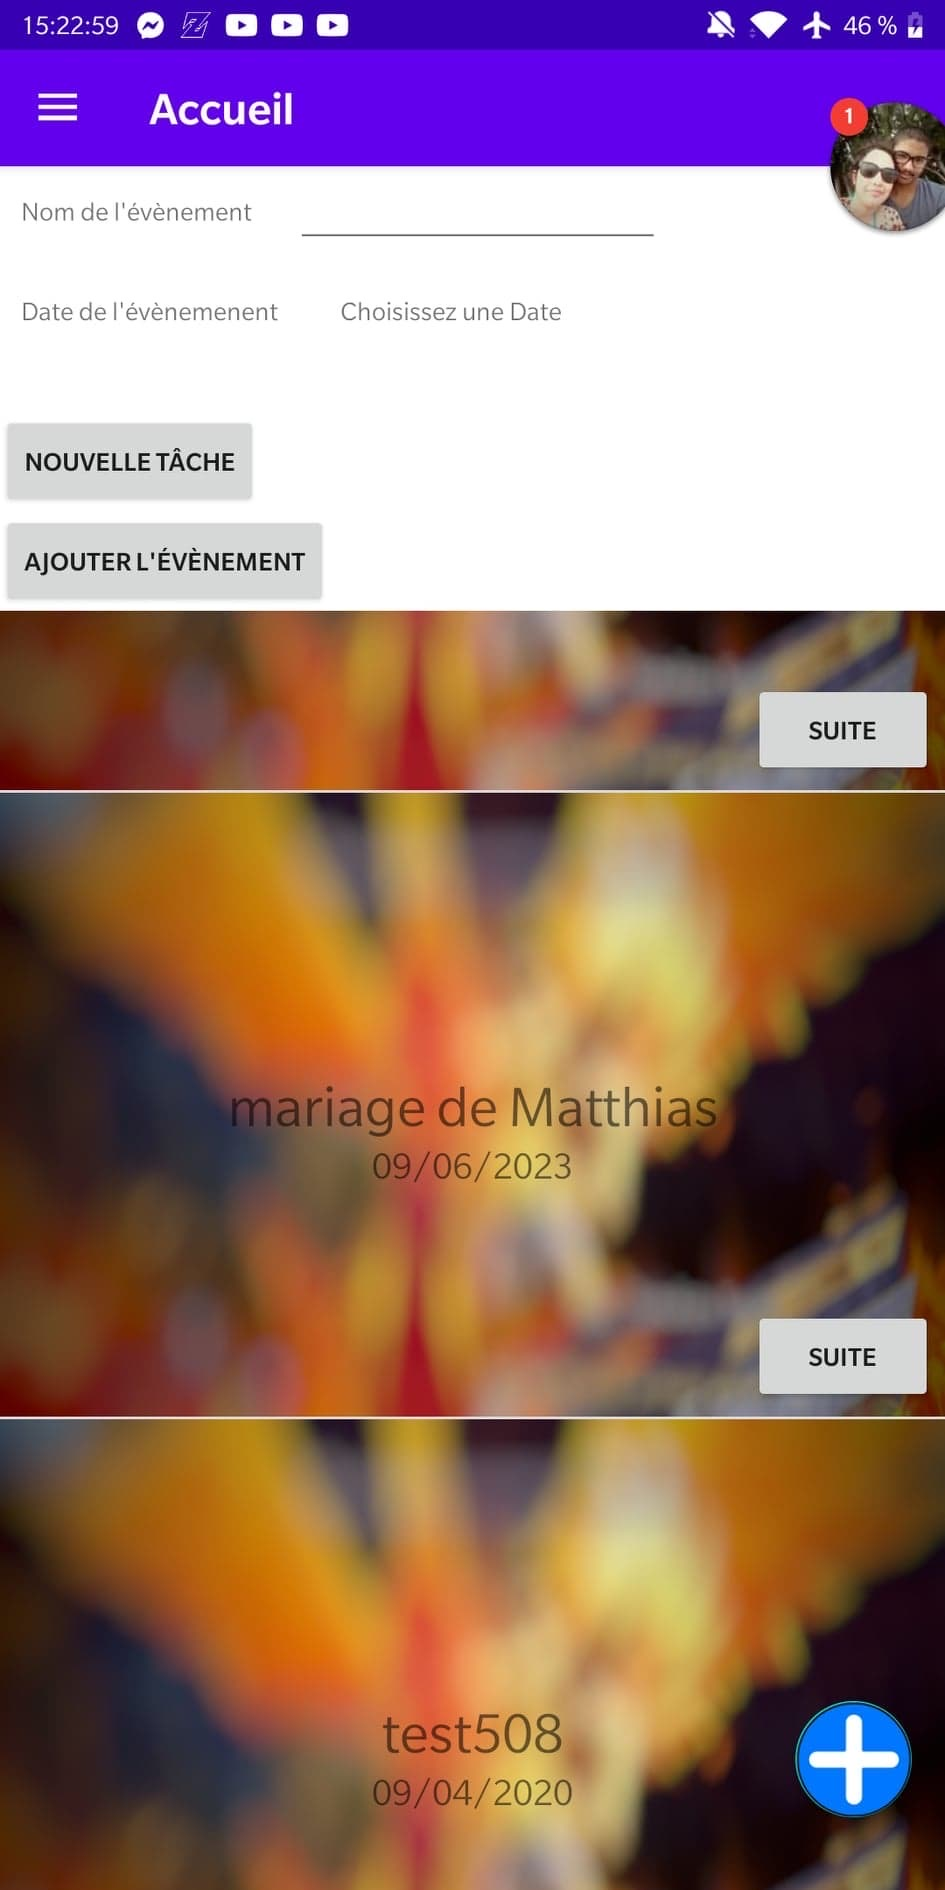
\includegraphics[scale=0.2]{SupperPosFrag}

\column{0.6\textwidth}
\begin{mybox}{Solution pour la superposition}
problème résolu avec les lignes de codes :$if(container != null){
container.removeAllViews()}$ 
\end{mybox}


\end{columns}
\end{frame}

\begin{frame}{Problème Rencontrés}


\begin{columns}

\column{0.5\textwidth}
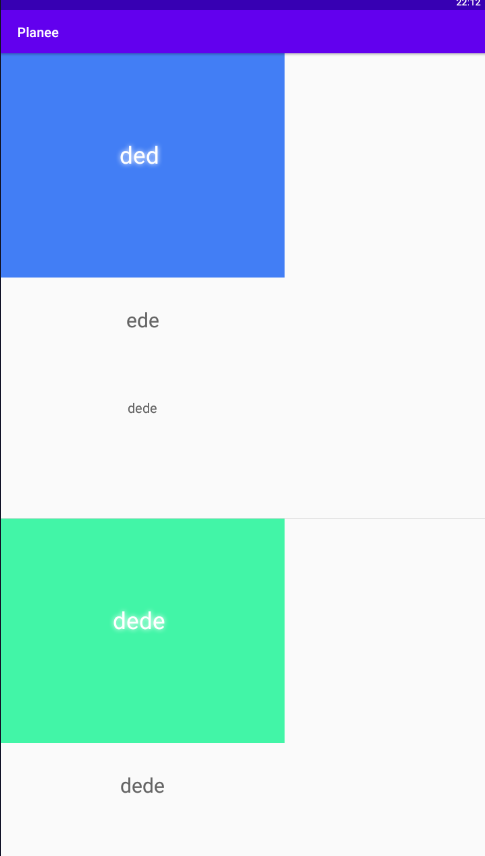
\includegraphics[scale=0.4]{BugLayout}

\column{0.6\textwidth}
\begin{mybox}{Problèmes liés aux Layouts}
Problème de mise à l'échelle selon la taille de l'écran 
\end{mybox}


\end{columns}
\end{frame}




\begin{frame}{Problèmes rencontrés}

\begin{mybox}{Problèmes liés aux Notifications}
\begin{flushleft}
Un problème majeure s'est montré lors de la création 
des notifications.Selon la version d'Android utilisée il fallait crée manuellement un "channel" afin de pouvoir diffuser la notification dessus.
\end{flushleft}
\end{mybox}
\begin{flushleft}
Si le channel n'était pas crée le message d'erreur suivant s'affiche dans le LogCat\\ 
\medskip
\begin{minipage}{0.48\linewidth}
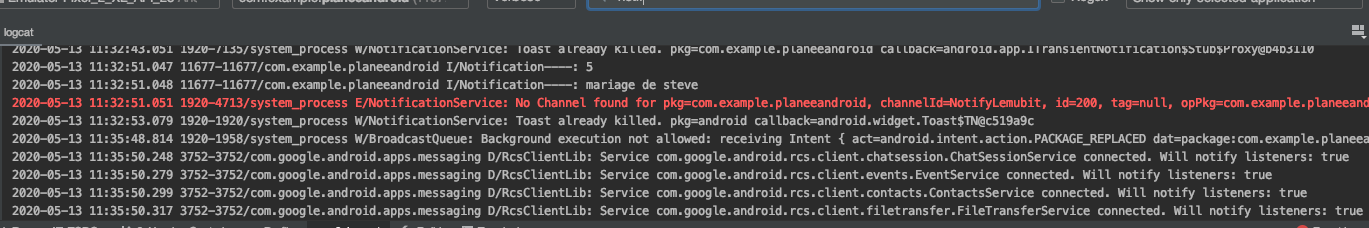
\includegraphics[scale=0.35]{LogcatNotif}
\end{minipage}%
\hfill
\end{flushleft}

\end{frame}


{%<--- Start local changes
\setbeamertemplate{navigation symbols}{}
\usebackgroundtemplate{
\includegraphics[height=\paperheight]{conclusion}}
\begin{frame}{Conclusion}
\end{frame}
}
\end{document}